The toy generation methods used for the global significance estimation in
\Cref{sec:global_significance} is described in the following.


\subsubsection{Generation of Observables}

The correlations between observables (i.e.~$n_{cb}$ in
\Cref{eq:likelihood_histfactory}) have to be quantified before proceeding with
the generation of toy experiments. Let $A$ and $B$ be the number of events
selected by two bins. Additionally, the marginal distributions of $A$ and $B$
are Poisson. The correlation between $A$ and $B$ is given by the overlap in the
kinematic region selected by both bins. The kinematic region selected by either
bin can be partitioned into three parts:
\begin{itemize}

\item The region selected by bin A but not B with number of
  events~$X_1$.

\item The region selected by bin A and B with number of events~$X_2$.

\item The region selected by bin B but not A with number of events~$X_3$.

\end{itemize}
The $X_i$ are distributed according to $\pois(\lambda_i)$ for $i = 1, 2, 3$ and
are mutually independent. Consequently, $A$ and $B$ can be written as
\begin{align*}
  A &= X_1 + X_2 \sim \pois(\lambda_1 + \lambda_2) \\
  B &= X_2 + X_3 \sim \pois(\lambda_2 + \lambda_3)
\end{align*}
and the linear correlation coefficient between $A$ and $B$ is given
by\footnote{$\cov(A,B) = \cov(X_1 + X_2, X_2 + X_3) = \cov(X_2, X_2) = \var(X_2)
  = \lambda_2$ from the independence of $X_1$, $X_2$, and $X_3$.}
\begin{align*}
  \rho_{AB} = \frac{\cov(A, B)}{\sqrt{\var(A)\var(B)}}
  = \frac{\lambda_2}{\sqrt{(\lambda_1 + \lambda_2) \cdot (\lambda_2 + \lambda_3)}} \,\text{.}
\end{align*}
This equation reflects the intuition that the overlap between bins, described by
$\lambda_2$, introduces a correlation between both observables. In the
following, the model described by $A$ and $B$ is referred to as the bivariate
Poisson model~\cite{teicher1954}.

An approximation of the correlation coefficients for all bin pairs in a given
channel can be obtained by estimating the parameters $\lambda_i$ using MC
simulation and CR data. Excerpts of the correlation matrix obtained in the
\hadhad channel are shown in~\Cref{fig:correlation_matrix_observables}. In
total, 144 bins are considered in the \hadhad channel; therefore, the full
correlation matrix is of dimension $144 \times 144$. Similar matrices are
obtained in the \lephad SLT and LTT SRs with dimension $193 \times 193$ and
$182 \times 182$, respectively.

A few features of the correlation matrix shown in
\Cref{fig:correlation_matrix_observables} are noted in the following:
\begin{itemize}

\item Off-diagonal elements of submatrices describing the correlation between
  observables belonging to the same PNN discriminant are zero due to bins being
  pairwise disjoint by construction.

\item The most background-like bins have correlation coefficients of about
  \SI{90}{\percent} or larger. This is due to events that are easily rejected by
  the PNN discriminants, which predominately populate the first bins.
  % A large correlation for such bins is expected, independent of the targeted
  % \mX, due events that are kinematically incompatible with resonant \HH
  % production. Examples for such events are ones where both \mMMC and \mBB are
  % far from \mH.

\item The observables of the most signal-like bins in the intermediate mass
  range (cf.~\Cref{fig:correlation_matrix_observables_medium}) have little
  correlation. In contrast, in the high mass regime
  (cf.~\Cref{fig:correlation_matrix_observables_high}) the observables of the
  most signal-like bins can have correlations of up to \SI{75}{\percent}. This
  is due to the inability of the PNN to distinguish between different signal
  hypotheses with large \mX.

\end{itemize}
The correlation matrices in the \lephad SLT and LTT channels show similar
features.

\begin{figure}[htbp]
  \centering

  \begin{subfigure}{\textwidth}
    \centering

    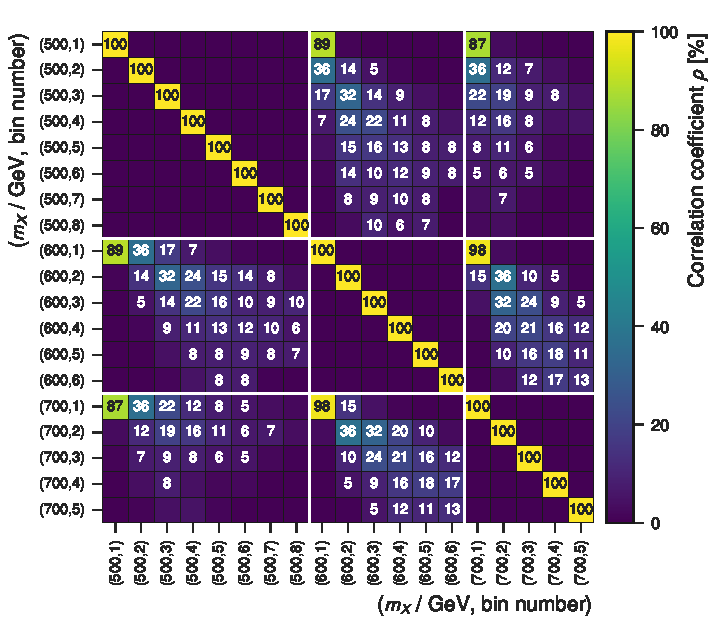
\includegraphics[scale=0.84]{global_significance/observable_correlations/corr_hadhad_medium}
    \subcaption{Submatrix for observables of the
      $\mX = 500, 600, 700\,\si{\GeV}$ PNN discriminants}%
    \label{fig:correlation_matrix_observables_medium}
  \end{subfigure}

  \begin{subfigure}{\textwidth}
    \centering

    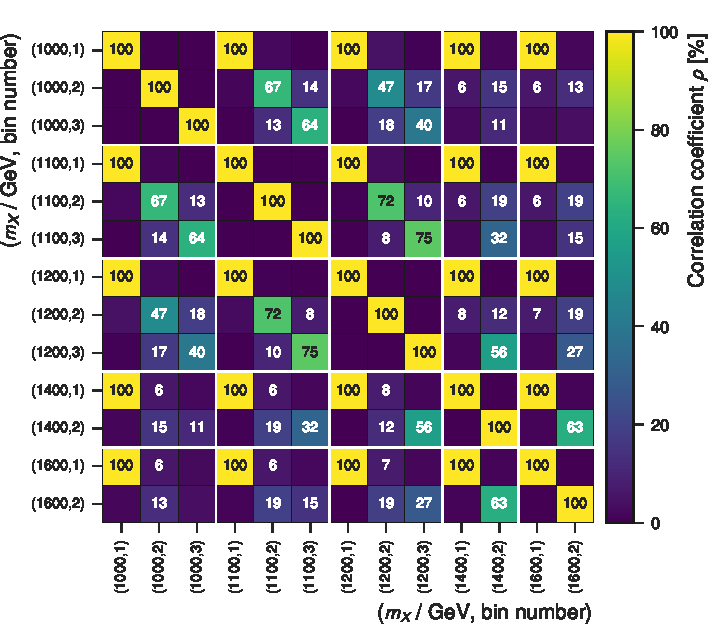
\includegraphics[scale=0.84]{global_significance/observable_correlations/corr_hadhad_high}
    \subcaption{Submatrix for observables of the
      $\mX = 1000, 1100, 1200, 1400, 1600\,\si{\GeV}$ PNN discriminants}%
    \label{fig:correlation_matrix_observables_high}
  \end{subfigure}

  \caption[Estimate of the correlation matrix between observables in the \hadhad
  channel.]{Estimate of the correlation matrix between observables in \hadhad
    channel. Two submatrices of the full matrix ($144 \times 144$) are
    shown. Bins are enumerated in increasing order of the signal probability
    according to the PNN discriminant (i.e.\ bins numbered with 1 contain the
    most background-like events). Cells are annotated if the correlation
    coefficient is larger than or equal to \SI{5}{\percent}. Off-diagonal
    elements with a correlation coefficient of \SI{100}{\percent} are due to
    rounding.}%
  \label{fig:correlation_matrix_observables}
\end{figure}

The toy generation for the global significance estimation needs to fulfil
certain requirements. First, the model needs to reproduce the marginal
distributions of the observables, i.e.\ Poisson distributions with mean
parameters equal to the number of events predicted by the nominal background
model.
% such that the distribution of the discovery test statistic for individual
% tests at fixed \mX can be reproduced.
Second, it needs to model the dependencies between observables due to the
overlap in the kinematic regions selected by bins.
% to account for the overlap in the kinematic region selected between all bin
% pairs.

A multivariate extension of the bivariate Poisson distribution would fulfil
these requirements; however, such a model becomes intractable due to the large
number of observables considered and the presence of negatively weighted events
in the background estimate.
% \footnote{In the absence of negatively weighted events, toy experiments can be
% generated by drawing a random weight from $\pois(w_i)$ for every event used
% for background estimation with event weight~$w_i$.}
Instead, a model based on the mathematical framework provided by Sklar's
theorem~\cite{Sklar1959FonctionsDR} is adopted, which can be used to factorise
the marginal distributions from the dependency structure of the observables. A
review of similar approaches of modelling multivariate count data is given in
Ref.~\cite{10.1002/wics.1398}.

Sklar's theorem states, see for example Ref.~\cite{nelsen}, that any
$n$-dimensional joint distribution function $H$ can be decomposed into $n$
marginal distribution functions $F_1, \dots, F_n$ and an $n$-dimensional copula
$\mathcal{C}$. The copula $\mathcal{C}$ is an $n$-dimensional distribution
function, $\mathcal{C}: [0, 1]^n \rightarrow [0, 1]$, with uniform marginal
densities that describes the dependencies between random variables. The joint
distribution can be expressed as
\begin{align*}
  H(x_1, \dots, x_n) = \mathcal{C}(F_1(x_1), \dots, F_n(x_n))
\end{align*}
according to the theorem.

For the task of generating toy experiments, the only missing piece is the
functional form of the copula since the marginal distributions are known from
the nominal background model. The bivariate Poisson distribution can be
approximated by a bivariate Normal distribution provided the means, $\lambda_i$,
are not too small. This suggests that the copula of a multivariate Normal
distribution might be a suitable approximation to model the dependencies between
observables. This copula, referred to as the Gaussian copula, can be derived
using the ``inversion method'' described in Ref.~\cite{nelsen} and is given by
\begin{align}
  \mathcal{C}_{\myvec{R}}(u_1, \dots, u_n) = \Phi_{\myvec{R}}(\Phi^{-1}(u_1), \dots, \Phi^{-1}(u_n)) \,\text{,}
  \label{eq:gaussian_copula}
\end{align}
where $\Phi_{\myvec{R}}$ is the CDF of the multivariate Normal distribution with
zero mean and covariance equal to the correlation matrix~$\myvec{R}$ and
$\Phi^{-1}$ is the quantile function of the univariate Standard Normal
distribution.

The parameters $\myvec{R}$ of the Gaussian copula are estimated by the
correlation matrices derived with the bivariate Poisson model. This
approximation is investigated empirically in two dimensions by comparing
simulated results of the bivariate Poisson model and a copula-based model. The
dependence of two observables $A$ and $B$ is illustrated in
\Cref{fig:copula_model_comparison} for both models in terms of the conditional
mean and variance of $B$ given $A = a$. This comparison is performed, instead of
a direct comparison of joint distribution functions, to better illustrate the
subtle differences between both models. The comparison yields the following
findings:
\begin{itemize}

\item The conditional mean of $B$ given $A = a$ agrees well between models, even
  when considering bin pairs with the lowest $\lambda_i$ relevant for the
  analysis.

\item The conditional variance of $B$ given $A = a$ illustrates that both models
  are not equivalent, however. For bin pairs with small $\lambda_i$, the
  variance of the distribution of $B$ for fixed $A = a$ differs by up
  \SI{15}{\percent} to between both models.

\item In the case of disjoint bins (not shown in the figure) the bivariate
  Poisson model and copula-based model are identical.

\end{itemize}

\begin{figure}[htbp]
  \centering

  \begin{subfigure}{\textwidth}
    \centering
    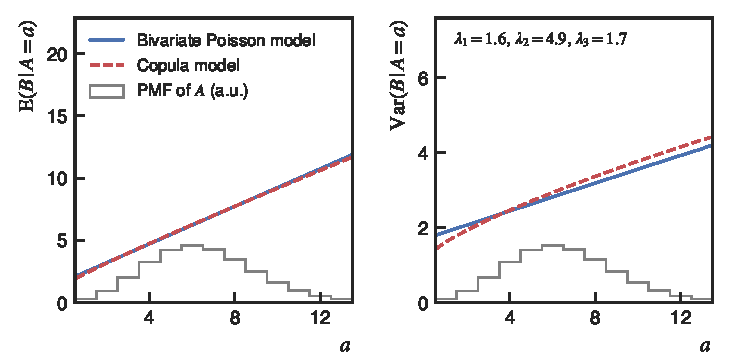
\includegraphics[scale=0.94]{global_significance/model_comparison/comparison_example_1}
    \subcaption{Most signal-like bins of the $\mX = \SI{1100}{\GeV}$ and
      $\mX = \SI{1200}{\GeV}$ PNN discriminants
      ($\rho_{AB} = \SI{75}{\percent}$).}
  \end{subfigure}

  \begin{subfigure}{\textwidth}
    \centering
    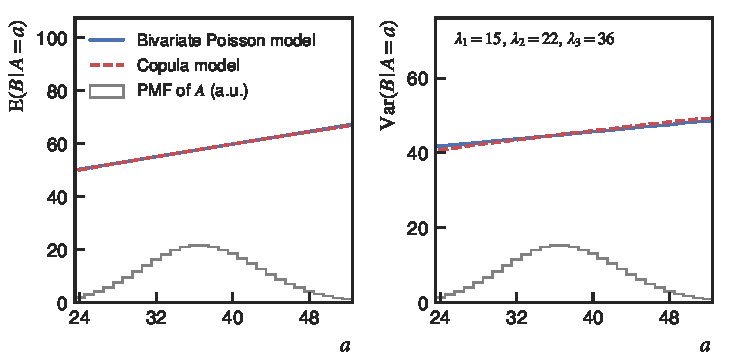
\includegraphics[scale=0.94]{global_significance/model_comparison/comparison_example_3}
    \subcaption{Second bin of the $\mX = \SI{1000}{\GeV}$ and second bin of the
      $\mX = \SI{1200}{\GeV}$ PNN discriminant
      ($\rho_{AB} = \SI{47}{\percent}$).}
  \end{subfigure}

  \begin{subfigure}{\textwidth}
    \centering
    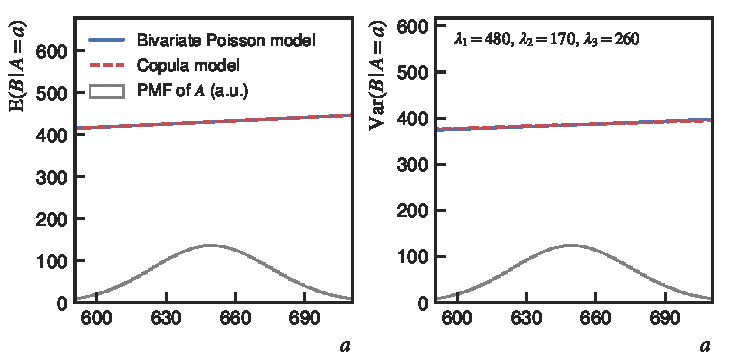
\includegraphics[scale=0.94]{global_significance/model_comparison/comparison_example_4}
    \subcaption{Third bin of the $\mX = \SI{500}{\GeV}$ and second bin of the
      $\mX = \SI{600}{\GeV}$ PNN discriminant
      ($\rho_{AB} = \SI{32}{\percent}$).}
  \end{subfigure}

  \caption[Comparison of the bivariate Poisson model and a model consisting of
  two Poisson marginal distributions linked by a Gaussian copula.]{Comparison of
    the bivariate Poisson model and a model using the Gaussian copula defined by
    $\rho_{AB} = \lambda_2 / \sqrt{(\lambda_1 + \lambda_2) \cdot (\lambda_2 +
      \lambda_3)}$ and marginal distributions given by
    $A \sim \pois(\lambda_1 + \lambda_2)$ and
    $B \sim \pois(\lambda_2 + \lambda_3)$. The conditional mean (left) and
    variance (right) of $B$ given $A = a$ is shown to illustrate the dependence
    of both random variables. Three different scenarios with varying $\lambda_i$
    and $\rho_{AB}$ are shown, which are chosen from bin pairs in the \hadhad
    channel. The probability mass function (PMF) of $A$ is overlayed in
    arbitrary units (a.u.).}%
  \label{fig:copula_model_comparison}
\end{figure}

With these simplifying assumptions, observables can be randomly generated using
the copula-based model. The following algorithm is employed to draw a vector of
random variates $\myvec{x} = (x_1, \dots, x_n)$ from the joint distribution
described by the Gaussian copula and marginal distributions~\cite{nelsen}:
\begin{enumerate}

\item Draw a vector of random variates $\myvec{u} = (u_1, \dots, u_n)$ from the
  distribution described by $\mathcal{C}_{\myvec{R}}$.

  The vector $\myvec{u}$ is obtained by generating random variates
  $\myvec{n} = (n_1, \dots, n_n)$ from the multivariate Normal distribution with
  zero mean and covariance matrix equal to $\myvec{R}$, followed by an
  element-wise application of the univariate Standard Normal CDF to $\myvec{n}$,
  that is, $u_i = \Phi(n_i)$ for $i = 1, \dots, n$. This procedure follows from
  the form of the Gaussian copula in~\Cref{eq:gaussian_copula}.

  In practice, the matrices $\myvec{R}$ that are considered here are singular
  due to multicollinearity between observables. This arises from 19 implicit
  constraints due to the requirement that the sum of observables is the same for
  all 20 discriminants in a given analysis channel, thus leading to 19 vanishing
  eigenvalues of $\myvec{R}$. Therefore, multivariate Normal random variates are
  generated in a lower dimensional space that removes the collinearity, followed
  by a back-transformation to the $n$-dimensional space. The required
  transformations are provided by an eigendecomposition of $\myvec{R}$.

\item Obtain $\myvec{x}$ by evaluating the quantile functions of the $n$
  marginal distributions at the values of $\myvec{u}$ from the previous step
  such that $x_i = F_{i}^{-1}(u_i)$ for $i = 1, \dots, n$. The marginal
  distribution functions are given by Poisson distributions with mean parameters
  corresponding to the nominal background prediction in a given bin.

\end{enumerate}
The multivariate count data generated with this method was inspected by
generating large samples of size $\mathcal{O}(10^6)$ showing agreement in terms
of the expected marginal distributions of the observables and closely
reproducing the pair-wise correlation coefficients estimated with the bivariate
Poisson model.


\subsubsection{Generation of Global Observables for the Barlow--Beeston Method}

This section describes the generation of global observables introduced by the
Barlow--Beeston method (i.e.~$m_{cb}$ in
\Cref{eq:likelihood_histfactory_constraints}).
%
% Global observables have to be fluctuated when estimating the global significance
% with toy experiments. This section will focus on the generation of the global
% observables related to the Barlow--Beeston method, previously described in
% \Cref{app:barlow_beeston}, that is used to include statistical uncertainties on
% the predicted background rates in the likelihood function. Due to the
% statistical nature of these uncertainties they cannot be neglected when
% estimating the global significances, particularly since these uncertainties have
% a large impact on the POI.
%
% Regarding global observables associated with the Barlow--Beeston method, similar
% considerations can be made as for the observables discussed in the previous
% section. The phase space selected by pairs of bins can partially overlap,
% leading to dependencies between the background rate predictions (from simulation
% and CR data) between bins. The random generation of these (global) observables
% is simplified, however, since resampling methods can be used.
%
The sample of simulated and CR events used for background estimation
% in all bins of the discriminants
is resampled using non-parametric bootstrap
methods~\cite{10.1214/aos/1176344552,efron1994introduction} to obtain replicas
that capture the statistical uncertainties and correlations of the background
predictions. Specifically, random weights $w_i^{\text{b}}$ drawn from $\pois(1)$
are assigned to all events~\cite{ATL-PHYS-PUB-2021-011}. These weights define
new background estimates~$\sum_{i} w_{i}^{\text{b}} \, w_i$ for all bins, where
$w_i$ is the nominal weight of event~$i$ and the sum goes over all events in a
given bin. Subsequently, the background estimate resulting from the bootstrap
procedure is translated into an effective number of unweighted events according
to
\begin{align*}
  m_{cb} = \frac{1}{s_{cb}} \sum_{i} w_{i}^{\text{b}} \, w_i \,\text{,}
\end{align*}
with a scaling factor $s_{cb} = \sum_i w_i^2 / \sum_i w_i$
(cf.~\Cref{app:barlow_beeston}) and the sums going over all events in bin~$b$ of
channel~$c$. Multiple toy experiments are generated by repeating the bootstrap
procedure.

In~\Cref{fig:comparison_bootstrap_poisson}, two exemplary distributions of
$m_{cb}$ in the \hadhad channel are shown. The figure compares the distribution
obtained from the bootstrap procedure with the distribution predicted by the
Barlow--Beeston method, i.e.\ the distribution of
$m_{cb} \sim \pois(\tau_{cb})$. In general, both distributions are not expected
to agree perfectly since the Barlow--Beeston method itself is only an
approximation. Nevertheless, both approaches show decent agreement for scenarios
relevant to this analysis. Even in the case depicted
in~\Cref{fig:comparison_bootstrap_poisson_lowest_tau}, which corresponds to the
bin with the smallest effective number of unweighted events in the \hadhad
channel, the agreement is acceptable.

\begin{figure}[htbp]
  \centering

  \begin{subfigure}{0.485\textwidth}
    \centering

    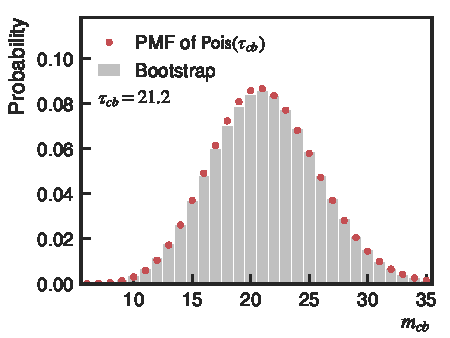
\includegraphics[width=0.98\textwidth]{global_significance/gamma_globs/gamma_obs_251}
    \subcaption{Most signal-like bin of the $\mX = \SI{251}{\GeV}$
      PNN discriminant in the \hadhad-channel.}%
    \label{fig:comparison_bootstrap_poisson_lowest_tau}
  \end{subfigure}\hfill%
  \begin{subfigure}{0.485\textwidth}
    \centering

    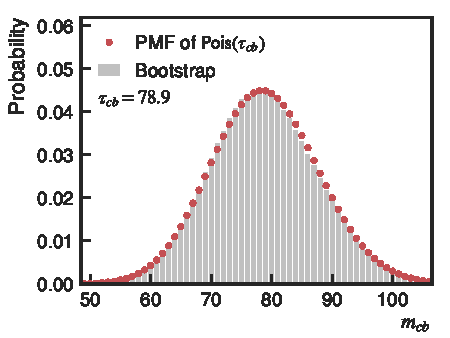
\includegraphics[width=0.98\textwidth]{global_significance/gamma_globs/gamma_obs_1000}
    \subcaption{Most signal-like bin of the $\mX = \SI{1000}{\GeV}$ PNN
      discriminant in the \hadhad-channel.}
  \end{subfigure}

  \caption[Distributions of $m_{cb}$ derived using a bootstrap procedure and
  predicted by the Barlow--Beeston method.]{Distributions of $m_{cb}$ derived
    using a bootstrap procedure (grey histogram) and predicted by the
    Barlow--Beeston method (red points). Two scenarios with different
    $\tau_{cb}$ are depicted, which are taken from the \hadhad channel.}%
  \label{fig:comparison_bootstrap_poisson}
\end{figure}


%%% Local Variables:
%%% mode: latex
%%% TeX-master: "../../phd_thesis"
%%% End:
